\documentclass[../thesis.tex]{subfiles}
\begin{document}
\chapter{Model Separation}
\label{ch:specific1}
In the original system, model information and simulation implementations deeply integrated, and model updates require changes to be made throughout the entire system. This prevents the system from having better flexibility. The goal of the new system is to accept mathematical models as input; based on the model input, the system should be able to dynamically adapt itself by creating corresponding data structures and function calls simulation. In this section, I aim to separate all model information from simulation methods and data structures. Through model separation, the future system users will be able to easily update or switch biological models while keeping the rest of the system untouched. 
\section{Methodology}
A new form of model representation is designed for model information in the new system. In this representation, the basis of the model consists of a list of species and list of reactions related to those species ($species\_list.hpp$ and $reaction\_list.hpp$, respectively). Each of the reaction has its specific $reaction\_id$. On top of those two files, there are two additional structures.  The first file, $reaction.cpp$, (Figure \ref{fig:reac1}) contains data structure describing the relations between species and reactions, which involve input, output and determining species of each reaction and their effects. The second file, $model\_impl.hpp$, (Figure \ref{fig:modelim1}) describes mechanisms of each reaction, which are the related active rates and concentration levels used in this reaction. Notice here that each function in this file is templated on two parameters and one of them is $reaction\_id$, and it will be useful later.\\
\begin{figure}[h]
\centering
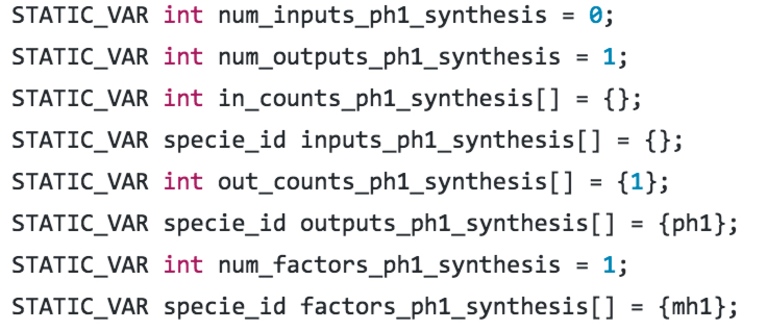
\includegraphics[width=0.6\textwidth]{reactioncpp}
\caption{Snippet of Code from $reaction.cpp$}
\label{fig:reac1}
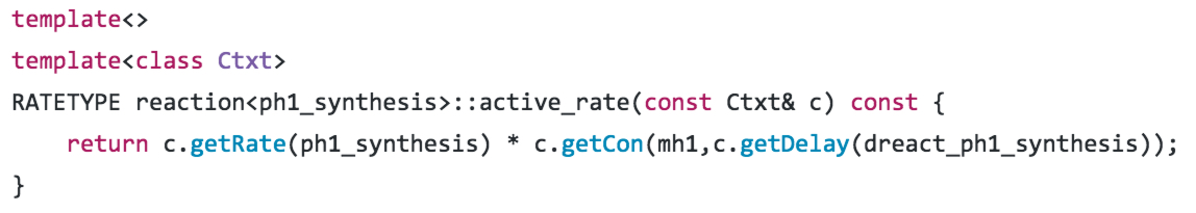
\includegraphics[width=0.9\textwidth]{modelimpl}
\caption{Snippet of Code from $model\_impl.hpp$}
\label{fig:modelim1}
\end{figure}
\\
Since the system is trying to dynamically create data structures and functions though this representation of model information, some level of polymorphism is required to accomplish this task. A common way to construct this class is to use virtual functions. Then, different kinds of reactions will specify different functions in order to calculate reaction rate. This is undesirable in our system, however, because all virtual functions provide only run-time polymorphism.  Since virtual functions are small, the overhead of looking up corresponding member function at runtime is high relative to the amount of work the functions do. In other words, the system will be much less efficient since those functions cannot be optimized during compile time. To overcome the loss of complier optimization, I introduced \textit{x-macros} into the system and define a reaction and species list as an enumerated list. Through \textit{x-macros}, resulting data structures and function calls can be generated during pre-processing, thus granting polymorphism while enjoying compiler optimization. Details of \textit{x-macros} usage will be clarified in the next section due to its close interaction with simulation. 
\section{Results}
In this section, we choose a much higher level of generalization of model information at the cost of not continuing to use design and manual optimization of the previous system. Usage of \textit{x-macros} provides enough compensation to the system to make generalization viable, though. It is important to note here that manual optimization of this particular section of the system is impractical. Manual optimization requires all data structures and functions to be static and written in the system before compilation. Yet the ultimate goal of the system is to keep simulation section independent of model input, thus allowing convenient model switch. Manual optimization is contradictory to the purpose of the study and the model information can only be restricted to a certain degree to include as many biological models as possible. As for the restriction imposed on model information currently, manual optimization in simulation is already completed and will be explained in detail in the next section.
\end{document}
